\documentclass[paper=letter, fontsize=12pt]{article}
\usepackage{geometry}
\geometry{margin=1in}
\usepackage{graphicx}
\graphicspath{{images/}}
\usepackage{amssymb}
\usepackage{enumitem}
\usepackage{amsmath}

%opening
\title{Compsci 571 HW4}
\author{Yilin Gao (yg95)}

\begin{document}

\maketitle
\section{Constructing Kernels}

\section{Reproducing Kernel Hilbert Spaces}

\section{Convexity and KKT Conditions}

\begin{enumerate}[label=(\alph*)]
	% 3a
	\item
	The Lagrangian function for the primal form is:
	
	$$
	\min L(\mathbf{w}, \mathbf{\eta}, \mathbf{\eta^*}, \mathbf{a}, \mathbf{b}, \mathbf{c}, \mathbf{d}) = \frac{1}{2} \Vert \mathbf{w} \Vert^2 + C \sum_{i = 1}^{n} (\eta_i + \eta_i^*) + \sum_{i = 1}^{n} a_i [y_i - \mathbf{w}^T \mathbf{x}_i - \epsilon - \eta_i]
	$$
	
	$$
	+ \sum_{i = 1}^{n} b_i[\mathbf{w}^T \mathbf{x}_i - y_i - \epsilon - \eta_i^*] - \sum_{i = 1}^{n} c_i \eta_i - \sum_{i = 1}^{n} d_i \eta_i^*
	$$
	
	It's KKT conditions are:
	
	\begin{itemize}
		\item Primal feasibility: 
		
		$$y_i - \mathbf{w}^T \mathbf{x}_i - \epsilon - \eta_i \leq 0, i = 1, \dots, n$$
		$$\mathbf{w}^T \mathbf{x}_i  - y_i - \epsilon - \eta_i^* \leq 0, i = 1, \dots, n$$
		$$\eta_i \geq 0, i = 1, \dots, n$$
		$$\eta_i^* \geq 0, i = 1, \dots, n$$ 
		
		\item Dual feasibility:
		
		$$a_i \geq 0, i = 1, \dots, n$$
		$$b_i \geq 0, i = 1, \dots, n$$
		$$c_i \geq 0, i = 1, \dots, n$$
		$$d_i \geq 0, i = 1, \dots, n$$
		
		\item Complementary slackness:
		
		$$a_i [y_i - \mathbf{w}^T \mathbf{x}_i - \epsilon - \eta_i] = 0,  i = 1, \dots, n$$
		$$b_i [\mathbf{w}^T \mathbf{x}_i  - y_i - \epsilon - \eta_i^*] = 0,  i = 1, \dots, n$$
		$$c_i \eta_i = 0,  i = 1, \dots, n$$
		$$d_i \eta_i^* = 0,  i = 1, \dots, n$$
		
		\item Lagrangian stationary:
		
		$$\nabla_{\mathbf{w} L} = \mathbf{w} - \sum_{i = 1}^{n} (a_i - b_i) \mathbf{x}_i = 0$$
		$$\nabla_{\mathbf{\eta} L} = C - \mathbf{a} - \mathbf{c} = 0$$
		$$\nabla_{\mathbf{\eta^*} L} = C - \mathbf{b} - \mathbf{d} = 0$$

	\end{itemize} 

	With these conditions, we can transform Lagrangian function into dual form:
	
	$$
	\max L(\mathbf{a}, \mathbf{b}) = \sum_{i = 1}^{n} (a_i - b_i) y_i - \epsilon \sum_{i = 1}^{n} (a_i + b_i) - \frac{1}{2} \sum_{i, j = 1}^{n} (a_i - b_i) (a_j - b_j) \mathbf{x}_i^T \mathbf{x}_j
	$$
	
	subject to 
	$$
	0 \leq a_i, b_i \leq C, i = 1, \dots, n
	$$
	
	% 3b
	\item
	Support vectors are the points $i$ such that $\vert y_i - \mathbf{w}^T \mathbf{x}_i \vert \leq \epsilon$.
	
	% 3c
	\item
	Increasing $\epsilon$ makes the model less likely to overfit. Because the model penalizes the points that have training error larger than $\epsilon$. If $\epsilon$ increases, the allowed/unpenalized training error increases, and the model tends to overfit less.
	
	% 3d
	\item
	Increasing $C$ makes the model more likely to overfit. $C$ is the penalty for each point that has training error larger than $\epsilon$. If the penalty increases, the model will try to make points have smaller training error, and thus overfits.
	
	% 3e
	\item    
	Assume we've computed the optimal dual variables as $\mathbf{a}^*$ and $\mathbf{b}^*$.
	
	From one of the KKT conditions, we can get the optimal primal variable is $\mathbf{w}^* = \sum_{i = 1}^{n} (a_i^* - b_i^*) \mathbf{x}_i$ .
	
	So for a new point $\mathbf{x}^{new}$, its evaluation is $f(\mathbf{x}^{new}) = \sum_{j = 1}^{p} w_j^* x_j^{new} = \sum_{j = 1}^{p} \sum_{i = 1}^{n} (a_i^* - b_i^*) x_{ij} x_j^{new} = \sum_{i = 1}^{n} (a_i^* - b_i^*) \mathbf{x}_i \cdot \mathbf{x}^{new }$.
\end{enumerate}

\section{SVM Implementation}
\begin{enumerate}[label=(\alph*)]
	%4a
	\item See \texttt{smv\_classifier.py}.
	
	%4b
	\item \textbf{Note: for questions (b) and (c), I use \texttt{sklearn.mode\_selection.train\_test\_split} to split the training and testing set with 2018 as the random seed. And I've noticed if I use \texttt{numpy} to generate indices with 2018 as the random seed and then split, the split is different.} Code for these 2 questions are in \texttt{q4.ipynb}.
	
	The accuracy of the classifier on testing data is 0.8636363636363636. The ROC curve is like following:
	
	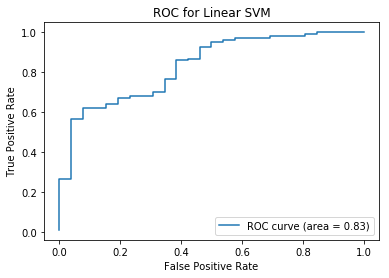
\includegraphics[scale=0.6]{q4b.png}
	
	The AUC on testing data is 0.8316400580551523.
	
	%4c
	\item For $\sigma^2 = 25$, the accuracy of the classifier on testing data is 0.8484848484848485. The ROC curve is like:
	
	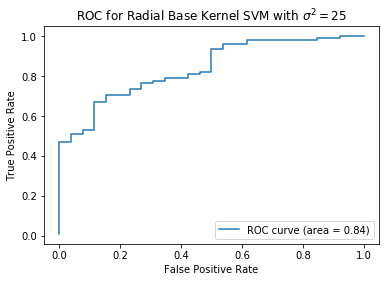
\includegraphics[scale=0.6]{q4c1.png}
	
	The AUC on testing data is 0.8388969521044993.
	
	For $\sigma^2 = 5$, the accuracy for the classifier on testing data is 0.7954545454545454. The ROC curve is like:
	
	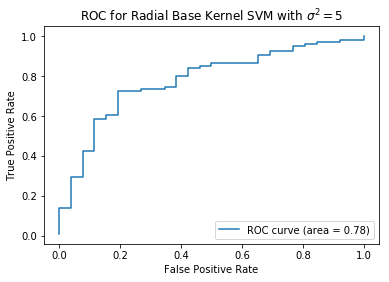
\includegraphics[scale=0.6]{q4c2.png}

	The AUC on testing data is 0.7790275761973875.
	
	The comparison between 2 $\sigma^2$ values suggests that for Gaussian kernel if we set $\sigma^2$ too small we may overfit.
\end{enumerate}

\end{document}
